\documentclass[a4paper,12pt,openany, DIV=calc, headsepline]{scrbook}
\usepackage[utf8]{inputenc}
%\usepackage[cp1250]{inputenc}
\usepackage[T1]{fontenc}
\usepackage[polish]{babel}
%\usepackage[fixlanguage]{babelbib}
%\selectbiblanguage{polish}
%\usepackage[T1]{polski}
%\usepackage{times}
\usepackage{amsmath}
%\usepackage{amssymb}
\usepackage{amsfonts}
\usepackage{amsthm}
\usepackage{lmodern}
%\usepackage{scrpage2}
\usepackage{natbib}
\usepackage{float}
\usepackage{algorithm2e}

\usepackage{caption}
\usepackage{subcaption}
\usepackage{graphicx}
\usepackage{geometry}
\usepackage{hyperref}
%\usepackage{subfigure}
%\usepackage{longtable}
%\usepackage{stmaryrd}
%\usepackage{wasysym}
%\usepackage{lscape}
\usepackage{url}
%\usepackage{calc}
%\usepackage{multirow}
%\usepackage{multicol}
\usepackage{enumerate}
\usepackage{makeidx}
%\usepackage{epstopdf}
\usepackage{setspace}
%\usepackage[usenames,dvipsnames]{pstricks}
%\usepackage{pst-eps} % For gradients
%\usepackage{pst-plot} % For axes
%


\newgeometry{tmargin=2.5cm, bmargin=2.5cm, lmargin=2cm, rmargin=2cm}
\doublespacing
\addcontentsline{toc}{chapter}{Wstęp}
%\singlespacing
\begin{titlepage}
\titlehead{\center{\LARGE Uniwersytet Ekonomiczny w Krakowie}\\
\vskip2mm
{\LARGE Wydział Zarządzania}\\
\vskip2mm
{\LARGE Katedra Statystyki}}

\author{{\LARGE \textbf{Zygmunt Zawadzki}}\\
numer albumu: 161509\\
Kierunek: Analityka Gospodarcza\\
Specjalność: Modelowanie i Prognozowanie}

\subject{Praca magisterska}
\title{Filtracja danych wysokiej częstotliwości}
%\dedication{Rodzicom}
%\subtitle{Short but sweet?}
\publishers{{\Large Opiekun naukowy: dr hab. Daniel Kosiorowski}}
\vskip2mm
\date{Kraków, 2015}
\end{titlepage}
\begin{document}

\maketitle

\tableofcontents
\chapter*{Wstęp}


W ostatnich latach coraz szerszą popularność zdobywają algorytmiczne fundusze inwestycyjne, w których decyzje o inwestycjach podejmowane są z wyłączeniem czynnika ludzkiego. Zastosowanie algorytmów pozwala znacząco skrócić czas analizy potrzebnej do podjęcia decyzji o zajęciu określonej pozycji rynkowej, dzięki czemu w danej chwili może być analizowany dużo szerszy portfel aktywów z wykorzystaniem bardziej złożonych modeli. 

Jednocześnie podejście algorytmiczne krytycznie zależy od jakości dostępnych danych. Ma tu zastosowanie zasada GIGO\footnote{GIGO - Garbage in-Garbage out} mówiąca, że nawet jeśli cały proces analizy jest poprawny, to przy danych złej jakości jakiekolwiek wnioski nie mają sensu. W przypadku, gdy inwestycji dokonuje człowiek niezależnie od tego, czy wspomaga się w procesie decyzyjnym analizą fundamentalną, techniczną, czy modelami statystycznymi, może on dokonać oceny jakości danych i dokonać ewentualnego czyszczenia, usuwając tym samym obserwacje odstające, które w innym przypadku zaburzyłyby wskazania użytych procedur. W przypadku algorytmicznym, z uwagi na ilość analizowanych instrumentów finansowych, jakakolwiek manualna ingerencja w dane jest znacząco utrudniona, bądź w ogóle nie możliwa. W takim przypadku jednym z rozwiązań jest wykorzystanie procedur odpornych, bądź odpowiednich algorytmów usuwania obserwacji odstających.

Pierwszym celem pracy jest prezentacja metody przygotowywania rzetelnych danych finansowych, które w później mogą być użyte w algorytmicznych strategiach inwestycyjnych, począwszy od etapu budowy, poprzez weryfikację, aż do rzeczywistego użycia na rynku. Główny nacisk rozważań zostanie położony na dane wysokiej częstotliwości, na których opiera się prezentowana metoda. Następnie przedstawione zostaną argumenty dotyczące występowania w danych finansowych obserwacji odstających, jak również rola statystyki odpornej w tej dziedzinie. Głównym celem pracy będzie prezentacja filtru pozwalającego usuwać obserwacje odstające w danych wysokiej częstotliwości.


\chapter{Wprowadzenie}

\section{Ocena jakość strategii inwestycyjnej}



Symulacja historyczna (ang. backtest) jest to  podstawowa procedura umożliwiająca ocenę jakość algorytmicznej strategii inwestycyjnej, na której opiera się w głównej mierze . 

W backteście, na podstawie danych historycznych generowane są hipotetyczne momenty otwarcia i zamknięcia pozycji, a następnie na ich podstawie wyznaczany jest szereg zwrotów dla strategii, który w dalszej części może służyć do weryfikacji jakość określonej strategii inwestycyjnej.

\section{Charakterystyka książki zleceń}

Kluczową konstrukcją w handlu na rynku finansowym jest książka zleceń. Zawiera ona wszystkie aktualne oferty kupna (Bid) i sprzedaży (Ask), dla danego instrumentu finansowego. W praktyce Bid i Ask używane są do określenia najlepszych cen kupna i sprzedaży. Sama książka zleceń składa się z poziomów, na których poszczególne zlecenia uporządkowane są malejąco dla ofert kupna i rosnąco dla ofert sprzedaży. W przypadku gdy pojawia się zlecenie kupna którego cena wykonania jest większa bądź równa od ceny dla dostępnych zleceń sprzedaży dochodzi do zawarcia transakcji, w przypadku zlecenia sprzedaży by doszło do transakcji cena zlecenia musi być niższa, bądź równa niż cena dostępnych zleceń kupna. Jeżeli pojawia się nowe zlecenia, które nie prowadzi do zawarcia transakcji trafia ono, na odpowiedni poziom książki zleceń.

W pewnych zastosowaniach prowadzi się analizę głębokości (liczby poziomów) książki zleceń. Taka analiza pozwala określić płynność dla danego instrumentu i ocenić wpływ jaki może mieć wprowadzenie zlecenia określonej wielkości. Dla przykładu - jeżeli na pierwszych dziesięciu poziomach znajdują się zlecenia o wolumenie jeden (oferta dotyczy jednej jednostki określonego instrumentu finansowego), wtedy by zawrzeć transakcję opiewającą na 10 jednostek instrumentu finansowego cena zlecenia będzie musiała być co najmniej równa cenie z dziesiątego poziomu, a w niższych poziomach cena może znacząco odbiegać od aktualnej najlepszej dostępnej ceny na rynku.

W wielu praktycznych sytuacjach jako cenę instrumentu przyjmuje się wartość najwyższej oferty kupna i najniższej oferty sprzedaży. Na ich podstawie wprowadza się następujące pojęcia, które będą używane w dalszej części pracy:

\begin{itemize}
\item \textbf{Bid} - najwyższa aktualnie dostępna cena kupna.
\item \textbf{Ask} - najniższa dostępna cena sprzedaży.
\item \textbf{Mid} - średnia cena instrumentu definiowana jako: (Ask+Bid)/2.
\item \textbf{Spread} - różnica pomiędzy Ask i Bid.
\end{itemize}

Na potrzeby pracy wprowadzone zostały również następujące określenia:
\begin{itemize}
\item \textbf{Tick} - wystąpienie zdarzenia na książce zleceń, będącego zmianą Bid, Ask, lub zawarciem transakcji.
\item \textbf{BidTick} - zmiana ceny Bid.
\item \textbf{AskTick} - zmiana ceny Ask.
\item \textbf{TransTick} - wystąpienie transakcji.
\end{itemize}

W niniejszej pracy analiza została ograniczona jedynie do pierwszego poziomu książki zleceń (Bid i Ask). Zlecenia modyfikujące niższe poziomy są pomijane.

\section{Metody przygotowywania danych do testów}


Finansowe dane wysokiej częstotliwości, kojarzone są głównie z handlem wysokiej częstotliwości (HFT), w którym pozycje trzymane są w bardzo krótkich interwałach czasowych, często nie przekraczających jednej sekundy. Zastosowanie tego typu danych wymaga posiadania odpowiedniej infrastruktury do przechowywania tego typu danych, jak i ich analizy. Dla przykładu jeden miesiąc HFD dla kontraktu fES.H15 zajmuje w postaci binarnej około 600 megabajtów, w postaci skompresowanej jest to ok. 60 megabajtów. Należy nadmienić, że ilość instrumentów finansowych może być liczona w dziesiątkach tysięcy.

Jednocześnie w wielu zastosowaniach, taka rozdzielczość danych nie jest w ogóle wymagana, a nawet może być szkodliwa (modelowanie zmienności i ryzyka). Dlatego też w praktyce w analizie cen instrumentów finansowych wykorzystywane są świeczki OHLCV (Open, High, Low, Close, Volume). Konstrukcja świeczki w klasycznym podejściu opiera się na agregacji wszystkich transakcji z okresu $t + \delta t$, gdzie $\delta$, określa przedział czasowy świeczki (np. godzina, 10 minut, etc.). Następnie pierwsza dostępna cena określa cenę otwarcia (Open), wartość najwyższa to High, najniższa Low, a ostatnia cena określa cenę zamknięcia (Close), zsumowany wolumen transakcji stanowi Volume. Tak przygotowane dane wykorzystywane są w dalszych etapach analizy finansowej (estymacja modeli zmienności, analiza techniczna i statystyczna etc.). Co więcej dane tej postaci są powszechnie dostępne w popularnych serwisach finansowych w internecie.

Przedstawione podejście oparte jedynie na wykonanych zleceniach, znajduje zastosowanie w przypadku płynnych aktywów, w których w danym okresie czasu dokonuje się wiele transakcji. W pewnych przypadkach może dojść do sytuacji w której w przedziale $\delta$, nie zawierane są żadne transakcje. Przykład takiej sytuacji prezentowany jest na rysunku \ref{fig:cottonTrans}, w godzinach od drugiej do trzynastej nie wystąpiły na przedstawionym instrumencie żadne transakcje. W przypadku próby budowy świeczek godzinowych w tym okresie wystąpiłyby brakujące dane.

Brak aktywności transakcyjnej nie oznacza jednak braku aktywności w ogóle. W dalszym ciągu na giełdę mogą przybywać zlecenia trafiające do książki zleceń, zmieniając tym samym rynkową wycenę instrumentu. Dlatego też wprowadza się metodę budowy świeczek OHLCV opartą na aktualnym stanie książki zleceń. W takim przypadku jako cenę otwarcia dla instrumentu, przyjmuje się wartość Mid w chwili $t$, następnie w okresie $<t,t + \delta t>$ monitoruje się wszystkie zmiany Ask i Bid, w celu znalezienia najwyższej i najniższej wartości Mid. Ceną zamknięcia jest Mid w chwili $t + \delta t$. Takie podejście pozwala lepiej uchwycić aktywność rynkową, co prezentuje rysunek \ref{fig:cottonOrder} przedstawiający BidTiki i AskTiki dla tego samego okresu który został przedstawiony na rysunku \ref{fig:cottonTrans}. Wyraźnie widać, że w okresie w którym nie występowały transakcje w dalszym ciągu instrument był aktywny i jego wycena rynkowa zmieniała się. Taka procedura budowy świeczek OHLCV pozwala znacząco zredukować ilość brakujących danych występujących w szeregu czasowym. 


\begin{figure}[H]
  \centering
  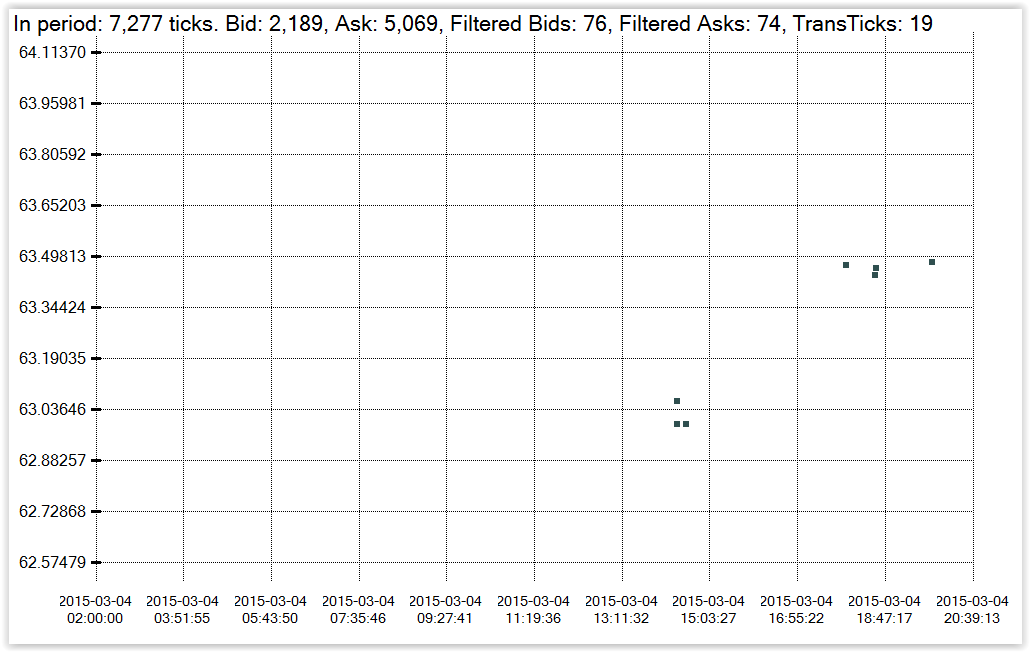
\includegraphics[scale=0.5]{wykresy/cottonTickH.PNG}
  \caption{Przypadel zakleszczenia się filtru. Po nagłym zwiększeniu się spreadu wszystkie kolejne ticki są usuwane.}
  \label{fig:cottonTrans}
\end{figure}

\begin{figure}[H]
  \centering
  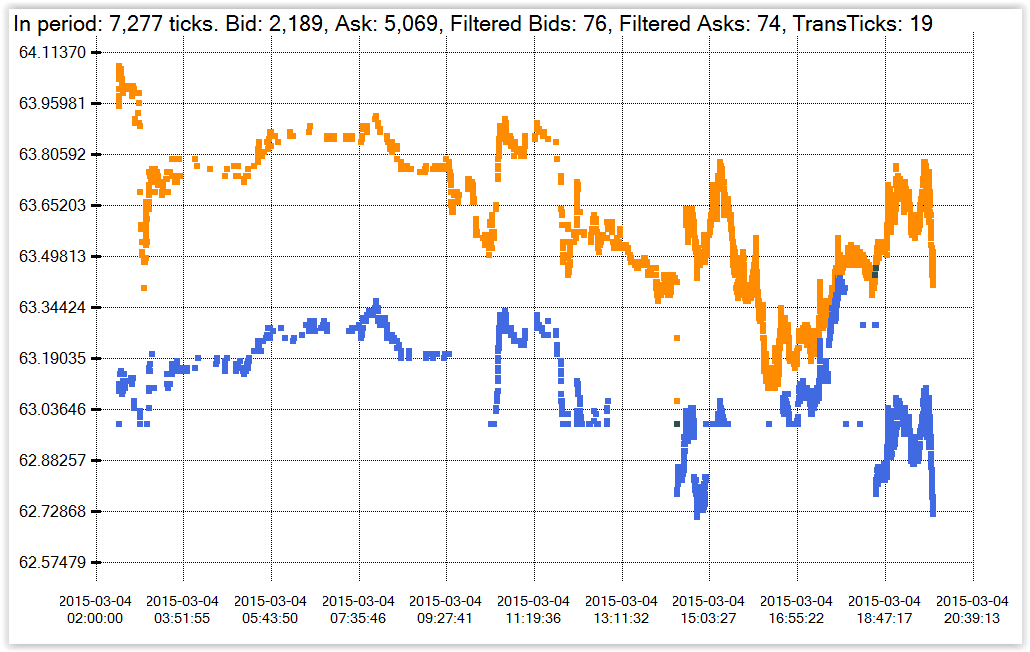
\includegraphics[scale=0.5]{wykresy/cottonOrderH.PNG}
  \caption{Przypadel zakleszczenia się filtru. Po nagłym zwiększeniu się spreadu wszystkie kolejne ticki są usuwane.}
  \label{fig:cottonOrder}
\end{figure}

\subsection{Przeprowadzanie symulacji historycznych z wykorzystaniem danych OHLCV}


Jednocześnie dla każdej świeczki OHLCV powinny zostać stworzone towarzyszące świeczki zbudowane z wykorzystaniem cen Bid i Ask. Zostaną one użyte w symulacjach historycznych (backtestach), do otwierania i zamykania pozycji. Ma to szczególne znaczenie w przypadku mniej płynnych aktywów, w których spread pomiędzy Bidem i Askiem może być bardzo znaczący - na rysunku \ref{fig:cottonOrder} w pewnych momentach stosunek spreadu do ceny Mid wynosi $0.7\%$, co oznacza, że cena wykonania zlecania kupna byłaby niedoszacowana o ok $0.35\%$, natomiast cena wykonania zleceń sprzedaży byłaby przeszacowana o tę wartość. Oznaczałoby to, że w testach pozycje zajmowane byłby po bardziej atrakcyjnych cenach niż były dostępne w rzeczywistości, a uzyskany wynik byłby przeszacowany. Ma to szczególne znaczenie w przypadku strategii o dużej częstotliwości transakcyjnej, w których efekt wykorzystania cen Mid (lub cen wyznaczonych na podstawie transakcji) jest dodatkowo potęgowany przez ilość transakcji, w skrajnych przypadkach, cały zysk określonej strategii inwestycyjnej może wynikać jedynie z tego efektu.

Dlatego też należy z dużą uwagą podchodzić do wyników algorytmicznych strategii inwestycyjnych przedstawionych w literaturze, gdyż prezentowane w nich wyniki mogą nie uwzględniać opisanego efektu związanego z użytymi danymi, a co za tym idzie są nie one możliwe do odtworzenia w poprawnych warunkach testowych. 

Jednocześnie dane wysokiej częstotliwości, w oparciu o które powinny być budowane szeregi czasowe do testów, są dostępne jedynie odpłatnie, co znacząco podnosi próg wejścia dla algorytmicznych funduszy inwestycyjnych.

%\subsection{Filtrowanie danych historycznych i danych na "żywo"}



\section{Charakterystyka danych wysokiej częstotliwości - stylizowane fakty}

Dane wysokiej częstotliwości charakteryzują się innymi własnościami niż klasycznie prezentowane własności finansowych szeregów czasowych. Co więcej, celem tej pracy jest wykorzystanie danych wysokiej częstotliwości do konstrukcji rzetelnych danych niższej częstotliwości, które będą użyteczne w dalszym modelowaniu statystycznym. Dlatego też pewne stylizowane fakty o klasycznie prezentowanych danych finansowych, takie jak grube ogony, czy grupowanie zmienności, w przypadku danych wysokiej częstotliwości nie mają w zasadzie znaczenia, lub nie mają znaczącego wpływu na cel pracy. 

By lepiej przedstawić charakterystykę HFD prezentowane są pewne stylizowane fakty uzyskane w trakcie prac z tymi danymi.

\subsection{Nierówne odstępy czasowe pomiędzy danymi}

Dane napływają w nieregularnych odstępach czasowych, silnie uzależnionych od aktualnej godziny sesji.

\subsection{Różnorodna częstotliwość zdarzeń}

Aktywność na książce zleceń w zależności od instrumentu charakteryzuje się bardzo różną intensywnością. Dla instrumentu przedstawionego na rysunku \ref{fig:cottonOrder} w okresie osiemnastu godzin doszło do 7277 zdarzeń, co daje około jedno zdarzenie na 10 sekund. Natomiast dla kontraktu E-Mini S\&P 500 przedstawionego na rysunku \ref{fig:spticks} w okresie 46 minut doszło do 200000 zdarzeń, co daje około 72 zdarzenia na sekundę.

\begin{figure}[H]
  \centering
  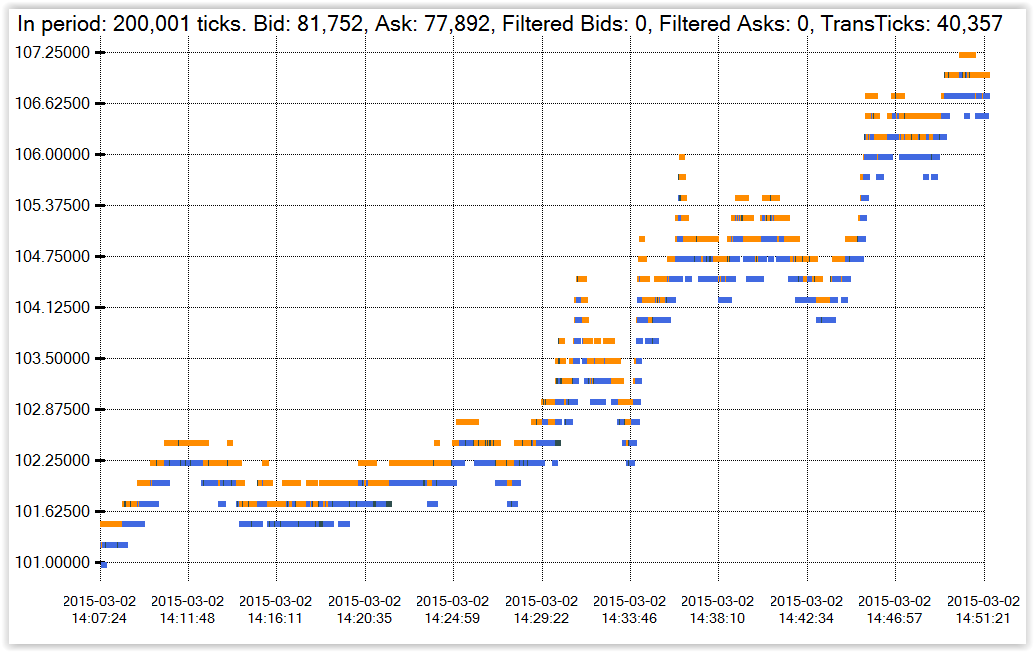
\includegraphics[scale=0.5]{wykresy/fESH.PNG}
  \caption{fESH.}
  \label{fig:spticks}
\end{figure}

Jednocześnie w większości przypadków ilość BidTick i AskTick jest zbliżona, jednak w pewnych sytuacjach mogą wystąpić znaczące różnice (np. w przypadku kontraktu zbliżającego się do wygaśnięcia). Taką sytuację prezentuje rysunek \ref{fig:fplh15}.

\begin{figure}[H]
  \centering
  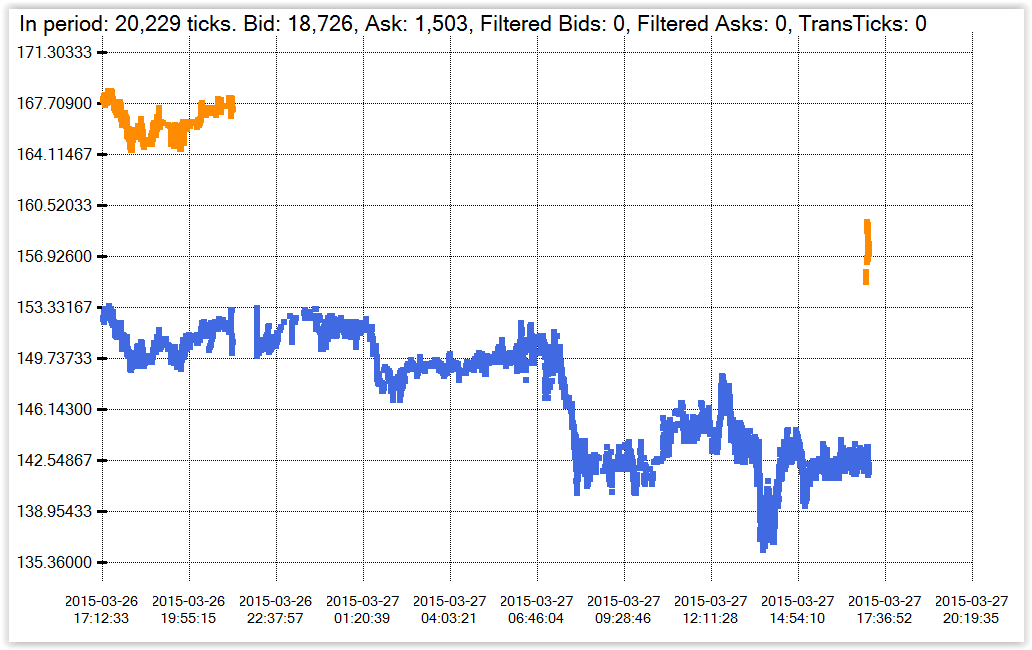
\includegraphics[scale=0.5]{wykresy/fplh15.PNG}
  \caption{fESH.}
  \label{fig:fplh15}
\end{figure}

\subsection{Występowanie spreadu}

Z faktu konstrukcji książki zleceń wynika iż, nie jest możliwe by Bid był większy od Ask, gdyż w takiej sytuacji dochodzi do zawarcia transakcji. Jednakże z faktu, że dane mogą przychodzić asynchronicznie ten warunek nie zawsze musi być spełniony. Rysunek \ref{fig:fpah15} prezentuje taką sytuację, w której $Bid > Ask$, mimo że nie doszło do żadnej transakcji. Należy zaznaczyć, że stworzony na potrzeby pracy program do wizualizacji HFD, w danym punkcie czasowym zaznacza to zdarzenie które miało miejsce pierwsze. Oznacza to, że w przypadku w którym pojawiają się dwa Ticki o tym samym znaczniku czasowym i cenie, kolor na wykresie będzie odpowiadał pierwszemu z nich. Najbardziej wiarygodnym wyjaśnieniem tej sytuacji jest anulowanie zlecenia zaznaczonego w punkcie A, jednak informacja na ten temat dostępna jest dopiero później. Całe zdarzenie miało miejsce w przedziale czasowym mniejszym niż jedna sekunda.

Sam spread podlega znaczenie mniejszym wahaniom niż same wartości Bid i Ask.

\begin{figure}[H]
  \centering
  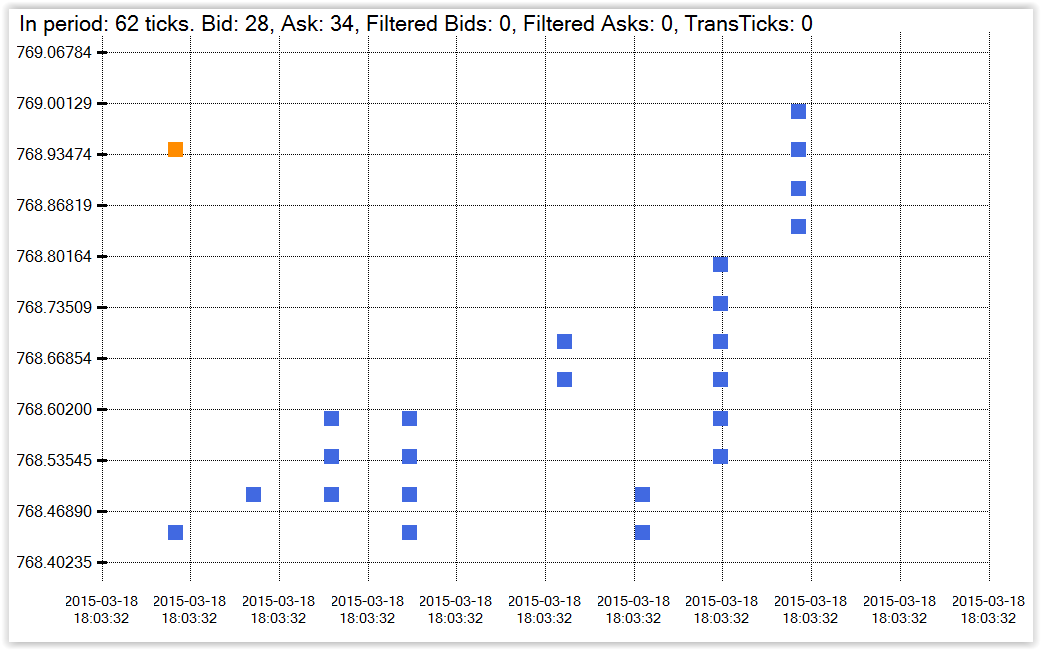
\includegraphics[scale=0.5]{wykresy/fpah15.PNG}
  \caption{fESH.}
  \label{fig:fpah15}
\end{figure}

\chapter{Obserwacje odstające w HFD}

\section{Obserwacje odstające w finansach}

Obserwacje odstające mogą mogą w pewnym stopniu być łączone z różnorodnymi błędami grubymi, dla przykładu obserwacja odstająca może pojawić się na etapie przepisywania danych poprzez przesunięcia przecinka, błędu w odczycie skali miernika itp. Jednakże definiowanie odstawania poprzez występowanie błędów grubych jest niewystarczające, gdyż w pewnych sytuacjach obserwacje mogą być w pełni poprawne, jednak ich użycie może znacząco zaburzyć wykonywane analizy. Przykładem takiej sytuacji mogą być dzienne zwroty dla pary walutowej EURCHF które prezentuje rysunek \ref{fig:eurchf}. Do dnia 14 stycznia 2015 roku dzienne zwroty zawierały się w przedziale od $-0.19\%$, do $0.26\%$. Natomiast od 16 stycznia ten przedział rozszerzył się do $(-1.1 \%; 3\%)$. Obserwacja z dnia 15 stycznia wynosi aż $-18.4\%$. W przypadku prostej, wizualnej analizy obserwacji w celu wykrycia obserwacji odstających taka wartość mogłaby zostać uznana za błąd polegający właśnie na przesunięciu przecinka, jednak jest to wartość całkowicie poprawna, która wynikła ze zdarzenia które miało miejsce w tym dniu. 15 stycznia 2015 roku Bank Centralny Szwajcarii ogłosił, iż przestanie bronić ustalonego kursu Franka wobec Euro, co spotkało się z bardzo gwałtowną reakcją inwestorów na całym świecie. Jednak mimo tego, iż ta obserwacja jest w pełni prawdziwa, znacząco odbiega od reszty obserwacji, a powtórne wystąpienie wartości na podobnym poziomie jest skrajnie nieprawdopodobne (wynikało ono z kompletnego zaskoczenia uczestników na rynku). Użycie takiej obserwacji w analizach dotyczących ryzyka (np. przy estymacji wartości zagrożonej), może prowadzić do znaczącego przeszacowania ryzyka w przyszłych okresach.

Dlatego też na potrzeby pracy obserwacja odstająca będzie definiowana jako obserwacja która w relacji do większości próby budzi zaskoczenie \citep{Ripley2004}. 

\begin{figure}[H]
  \centering
  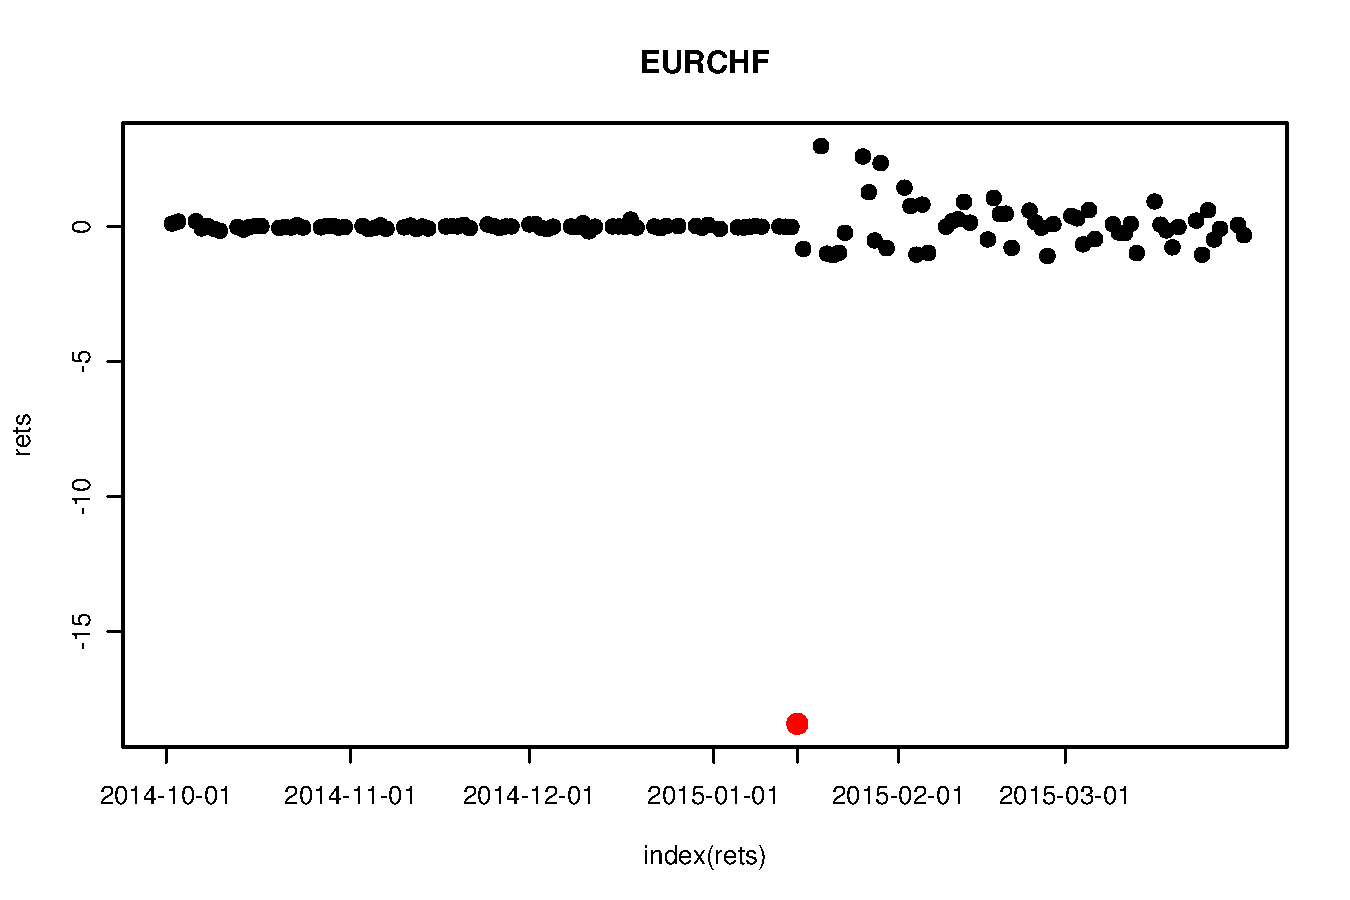
\includegraphics[scale=0.5]{wykresy/EURCHF}
  \caption{Dzienne zwroty na parze walutowej EURCHF. Obserwacja z dnia 2015-01-15 wyraźnie odbiega od reszty wartości.}
  \label{fig:eurchf}
\end{figure}


\section{Zastosowanie metod statystyki odpornej}

Każda procedura statystyczna konstruowana jest przy założeniu spełnienia określonych założeń, co do mechanizmu generującego dane. Przykładowo, dane generowane są przez rozkład normalny, a obserwacje są niezależne. Niestety w praktycznych przypadkach bardzo często nie można zapewnić iż wymagane przez procedurę założenia są spełnione. W takich przypadkach dalsze wnioskowanie statystyczne może być nieuprawnione, gdyż albo nieznane są w ogóle własności tych procedur, albo wymagania co do jakości uzyskanych estymatorów (obciążenie, efektywność, etc.) są niemożliwe do spełnienia.

Podejście proponowane przez statystykę odporną ma na celu prezentację procedur dających wiarygodne oszacowania nie tylko w przypadku, gdy dane generowane są przez zakładany rozkład, lecz również w przypadku gdy rozkład generujący dane odbiega od zakładanego. Odporna procedura statystyczna powinna dawać wiarygodne oszacowania również w przypadku gdy analizowany zbiór danych zawiera obserwacje odstające\citep{Van:2000}. Przykłady użycia odpornej procedury statystycznej prezentują rysunki \ref{lad1} i \ref{lad2}.

\begin{figure}[H]
\begin{subfigure}[t]{0.45\textwidth}
  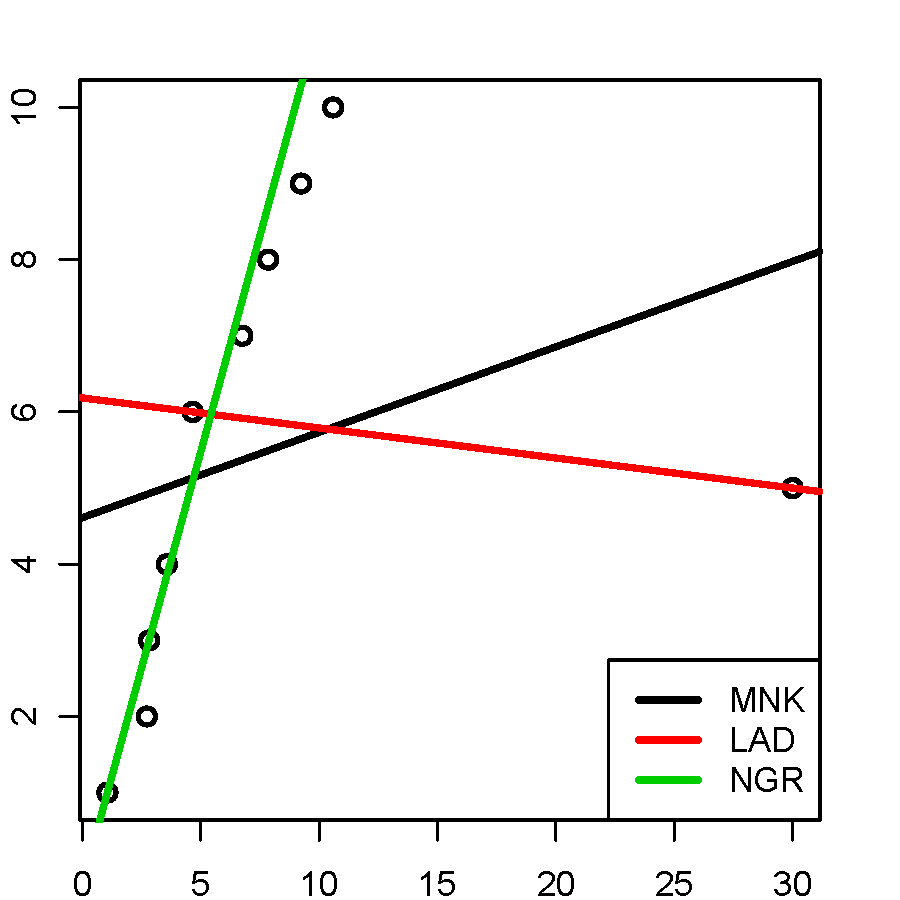
\includegraphics[width=\linewidth]{wykresy/ladout}
	\caption{Obserwacja odstająca ze względu na zmienną objaśniającą.}
	\label{lad1}  
\end{subfigure}
\begin{subfigure}[t]{0.45\textwidth}
  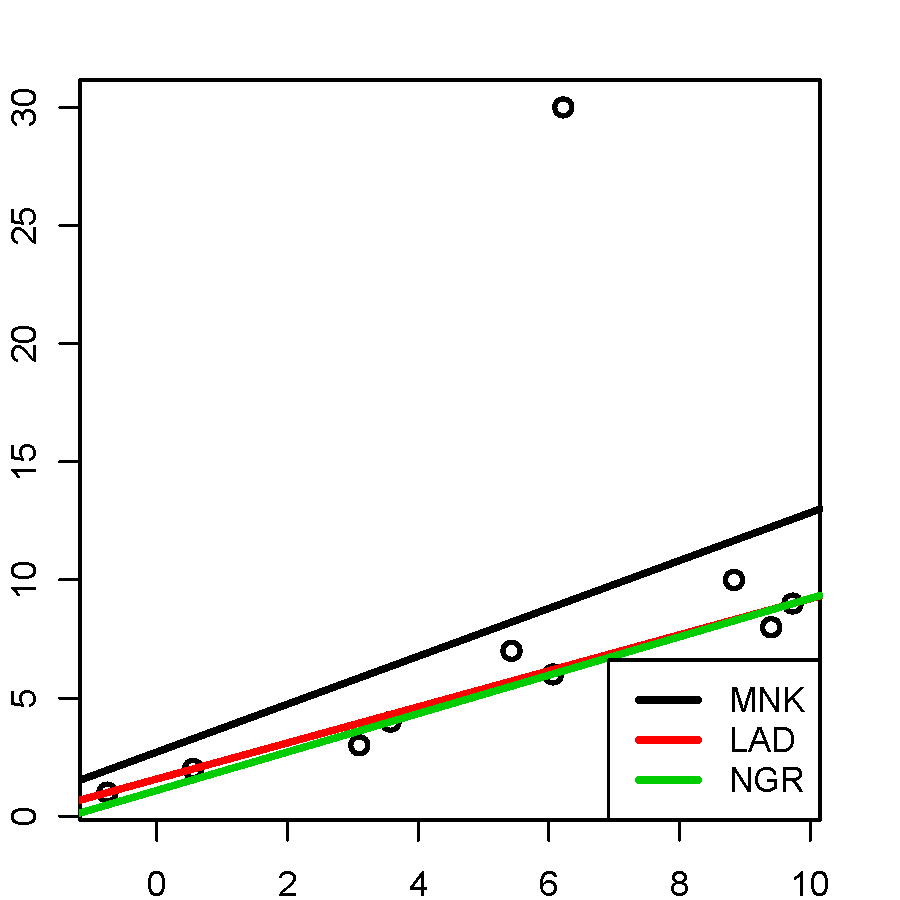
\includegraphics[width=\linewidth]{wykresy/ladouty}
  \caption{Obserwacja odstająca ze względu na zmienną objaśnianą.}
  \label{lad2}
\end{subfigure}
\caption{Przykładowe porównanie działania klasycznych (MNK i LAD) i odpornych (NGR - metoda największej głębi regresyjnej) estymatorów prostej regresji.}
\caption*{Źródło: Obliczenia własne - R Project}
\label{fig:lad}
\end{figure}

W przypadku prezentowanego problemu występowania obserwacji odstających w danych finansowych zastosowanie procedur statystyki odpornej wydaje się być uzasadnione, a nawet konieczne, jednak napotyka na pewne praktyczne problemy.

Procedury odporne są bardziej złożone obliczeniowo, od swoich klasycznych odpowiedników. O ile w przypadku potrzeby jednorazowej estymacji modelu z reguły różnice w czasie wykonywania nie są bardzo istotne, to specyfika testów jakim poddawane są strategie algorytmiczne wymaga wielokrotnej estymacji modelu, w której te różnice zyskują na znaczeniu, często nie pozwalając w ogóle na przeprowadzenie wiarygodnych testów w sensownym czasie. Dla przykładu, do wyznaczania wag dla portfela składającego się z 30 aktywów wykorzystywany jest klasyczny model Markowitza. Macierz kowariancji używana w obliczeniach wyznaczana jest na dwa sposoby, pierwszy wykorzystuje klasyczny estymator macierzy kowariancji, natomiast w drugim przypadku używany jest estymator MCD. W obu przypadkach brane jest pod uwagę ostatnie 504 obserwacje (dwa lata). Pojedynczy czas obliczeń w przypadku klasycznym wynosi 0.0003s, natomiast dla MCD około 1 sekundy. W symulacji na danych zawierających 10 lat, w której macierz kowariancji pomiędzy aktywami musi być obliczana dla każdego dnia, czas potrzebny na obliczenia estymatora klasycznego wyniesie łącznie ok 0.75 sekundy, natomiast dla estymatora MCD będą to aż 42 minuty. Zastosowanie estymatora odpornego tylko w tym jednym elemencie strategii sprawi, że czas obliczeń wydłuży się w znaczącym stopniu, przez co w danym okresie czasu będzie możliwe przetestowanie mniejszej ilości wariantów strategii. Równocześnie jednym z istotnych, kwestii jest zbadanie stabilności otrzymywanych wyników w pewnym otoczeniu parametrów strategii. W omawianym przykładzie mogłoby to wiązać się, ze sprawdzeniem jak zmieniają się wyniki w zależności od ilości obserwacji używanych do estymacji macierzy kowariancji. W takim przypadku, przy próbie sprawdzenie 50 różnych wariantów długości okna, obliczenia dla MCD zajęłyby około 50 godzin, przy czym jakiekolwiek inne obliczenia związane z logiką strategii są pomijane. 

Drugi aspekt związany jest z samą specyfiką testów strategii inwestycyjnych. W klasycznie prowadzonej analizie statystycznej po estymacji modelu, przeprowadza się jego weryfikację , poprzez testy dopasowania, lub zdolności prognostyczne, bądź klasyfikacyjne na odpowiednio przygotowanych zbiorach testowych (cross-walidacja). W przypadku strategii algorytmicznych, stosowane procedury statystyczne wykorzystywane są do generowania sygnałów określających pozycję jaką w danej chwili czasowej powinna zająć strategia. Sama pozycja może być utrzymywana przez określony czas symulacji (np. do zakończenia sesji w danym dniu symulacji), bądź do otrzymania sygnału zamknięcia, lub sygnału otwarcia pozycji przeciwnej. Następnie na podstawie szeregu cen dla instrumentu wyznaczana jest wartość pozycji i kolejne jej zmiany, aż do zamknięcia. Następnie na podstawie pozycji które zajmowała strategia generowane są krzywe kapitału strategii. Stosowanie procedur odpornych do wyznaczania sygnałów, po to by uchronić się przed obserwacjami odstającymi w danych w pewnym sensie legitymuje ich występowanie w szeregu. W takim przypadku mogą one mieć wpływ na wyznaczone wartości pozycji, a za tym idzie na wiarygodność wyniku prezentowanego przez strategię, co w dalszym kroku nakładałoby wymóg stosowania również odpornych metod do weryfikacji rezultatów strategii, uniemożliwiając stosowanie metod klasycznych , takich jak wskaźnik Sharpe.  

Dlatego też bardziej odpowiednim wydaje się usuwanie obserwacji odstających we wczesnym etapie symulacji, tak by nie miały one wpływu na stosowane procedury statystyczne, jak również wyznaczane wartości pozycji.

Jednocześnie stosowanie metod odpornych w celu zabezpieczenia się przed odstępstwami od rozkładu zakładanego przez procedurę statystyczną w dalszym ciągu jest uprawnione. Jedynie odstępstwa te, nie powinny objawiać się jako obserwacje odstające.

\chapter{Filtr}

\newcommand{\Spt}{\ensuremath{Sp_{t}} }

\newcommand{\MSpc}{\ensuremath{Sp_{t|t-1}} }
\newcommand{\MSpn}{\ensuremath{Sp_{t+1|t}} }
\newcommand{\MSpo}{\ensuremath{Sp_{t-1|t-1}} }

%% Czas
\newcommand{\ts}{\ensuremath{{t}} }
\newcommand{\tsl}{\ensuremath{{t-1}} }


%% Parametry filtru

\subsection{Główne założenia}

Zaprezentowany w dalszej części filtr został zbudowany w oparciu o cztery główne założenia.

\begin{itemize}
\item Dane mają być przetwarzane on-line. Oznacza to, że filtr musi działać bardzo szybko - tak by analiza pojedynczej obserwacji trwała krócej niż czas do pojawienia się kolejnej. Jednocześnie nie ma możliwości powrotu do obserwacji już przeanalizowanej (obserwacje nie są przechowywane).
\item Filtr powinien posiadać zdolność samo-naprawy w przypadku nieprzewidzianych zdarzeń. Niedopuszczalne jest "zakleszczenia się" filtru, jest to sytuacja w której wszystkie kolejne obserwacje z jednej, lub drugiej strony książki zleceń są odrzucane.
\item Koszt odrzucenia poprawnej obserwacji jest znacznie niższy, niż koszt przyjęcia za poprawną obserwacji odstającej. 
\item Filtr jest w pełni deterministyczny.
\end{itemize} 

Motywacją pierwszego założenia wynika z wymagań obliczeniowych. Filtr jest jednym z elementów który przez pewien moment przetrzymuje obserwację, zanim trafi ona do dalszej części silnika zarządzającego strategią inwestycyjną. Oznacza to, że zastosowanie filtra wprowadza pewne opóźnienie, które sprawia, że strategia otrzymuje dane już w pewien sposób zdezaktualizowane, przez co na pewne gwałtowne sytuacje rynkowe może zadziałać z zbyt późno. Jednocześnie jeżeli jeżeli czas na analizę musi być mniejszy niż okres pomiędzy obserwacjami, inaczej opóźnienie przesyłania danych z filtra będzie się nawarstwiać.

Należy również zwrócić uwagę, iż filtr będzie  stosowany równocześnie dla bardzo dużej liczby aktywów finansowych, przez co złożoność obliczeniowa jest dodatkowo potęgowana i może znacząco obciążać architekturę sprzętową. Z tego też powodu wprowadzono założenie, iż po jednokrotnym sprawdzeniu obserwacji nie ma już do niej powrotu, przez co znacząco minimalizowana jest złożoność pamięciowa realizowanego algorytmu.

Drugie założenie odnosi się do bardzo złożonych zjawisk występujących na rynku które mogą doprowadzić do sytuacji w której filtr w pewien sposób się ''zakleszczy'', co znaczy, że wszystkie kolejne obserwacje będą odrzucane. Przykłady takich zdarzeń rynkowych  pojawią się wraz z omówieniem wprowadzonych mechanizmów samo-naprawy w filtrze prezentowanym w niniejszej pracy.

Przypadek zakleszczenia się filtru jest bardzo groźny z punktu widzenia strategii, gdyż oznacza, że dane nie są przepuszczane do strategii, przez co niejako zostaje zatrzymane zarządzanie pozycją. Rozwiązaniem tego problemu jest stworzenie stosownego systemu ostrzeżeń, informującego o pojawiających się problemach (np. długa seria odrzuconych obserwacji). Jednak taki system wymaga nieustannego monitorowania (handel na międzynarodowym rynku odbywa się dwadzieścia cztery godziny na dobę), przez co może być nie praktyczny w realizacji. Dlatego też bardziej sensownym rozwiązaniem wydaje się wbudowanie pewnych metod naprawczych w sam filtr.






\subsection{Prezentacja algorytmu}

Oznaczenia:
\begin{itemize}
\item \ts - obecna chwila czasowa.
\item \tsl - czas ostatniego ticku.
\item \Spt  - spread w chwili \ts
\item \MSpc - średni spread w chwili \ts, obliczony na podstawie obserwacji do chwili \tsl.
\item \MSpn - średni spread w chwili \ts, po aktualizacji tickiem z tej chwili czasowej.
\item \MSpo - średni spread w chwili \tsl, po aktualizacji.
\end{itemize}

Parametry filtru:
\begin{itemize}
\item $minSpread$ Minimalny spread dla instrumentu.
\item $Multi$ - mnożnik średniego spreadu.
\item $min\phi$
\item $rmMulti$
\end{itemize}

W listingu \ref{FiltrBID} przedstawiono algorytm filtracji pojedynczej ceny bid. Algorytm filtracji ceny Ask jest analogiczny, jedyną różnicą są zamienione znaki $leq$ i $req$, dlatego też nie będzie omawiany.



\IncMargin{5em}
\begin{algorithm}
\KwData{\\
BidPrice - nowa cena bid.\\
time - czas wystąpienia tiku.}
\KwResult{Wartość logiczna - false w przypadku odrzucenia tiku}

\Spt = AskPrice - BidPrice; \tcc*[r]{AskPrice to ostatnia, nie odrzucona cena Ask.}



\nlset{Warunek 1}\label{War1}\If{$\Spt \leq SprMulti \cdot \MSpc$ lub \\ 
\nlset{Warunek 2}\label{War2}$BidPrice \leq AskPrice + CrossRange$ }
{
\nlset{Zabezpieczenie 1}\label{Zab1}	\Spt = lastDelAsk - BidPrice; \tcc*[r]{lastDelAsk to ostatnia, nie odrzucona cena Ask.}

	\If{$\Spt \leq SprMulti \cdot \MSpc$ lub \\ 
	$BidPrice \leq lastDelAsk + CrossRange$}
	{
		lastDelBid = BidPrice\\
\nlset{Zabezpieczenie 2}\label{Zab2} AskPrice = AskPrice + RmVal\\


	\Return{False}
	
	}
	
\nlset{Uwaga 1}\label{Uwaga1}	AskPrice = lastDelBid
	
}
\Return{True}

\caption{Algorytm filtracji cany Bid\label{FiltrBID}}
\end{algorithm}
\DecMargin{5em}

Warunek \ref{War1} testuje, czy nowy spread nie odbiega w znaczący sposób od średniego spreadu, co sugeruje obserwacje odstającą. 

Natomiast \ref{War2} ma na celu wychwycenie sytuacji, w której Bid przewyższa Ask w znaczący sposób. Samo zastosowanie warunku by $Bid < Ask$, jest nie wystarczające, gdyż dane pojawiają się w sposób asynchroniczny, przez co może dojść do sytuacji przedstawione na rysunku \ref{Fig:Cross} Dodatkowa granica \emph{CrossRange} pozwala wyłapać takie sytuacje, znacząco zmniejszając ilość niepotrzebnie odrzucanych ticków.

W linijce \ref{Zab1} spread przeliczany jest powtórnie, jednak z wykorzystaniem ostatniej odrzuconej ceny Ask. Powtórne sprawdzenie poprawności ticku pozwala zabezpieczyć działanie filtru w przypadkach dużych skoków cen. Scenariusz sytuacji występującej bez zastosowania takiego zabezpieczenia przedstawia rysunek \ref{fig:JUMP}. Jednocześnie może to prowadzić do zaakceptowania jako poprawne sytuacji w której krótko po sobie nastąpiły dwie obserwacje odstające (rysunek \ref{fig:NEXTOUT}).

Linija \ref{Zab2} jest kolejnym zabezpieczeniem przeciwko zakleszczeniu się filtru. W przypadku gdy dana cena Bid jest odrzucana, poprzez wartość RmVal następuje  podniesienie ceny Ask używanej do obliczeń wewnątrz filtru (sam filtr nie modyfikuje wartości tików). 

%\begin{figure}[H]
%  \centering
%  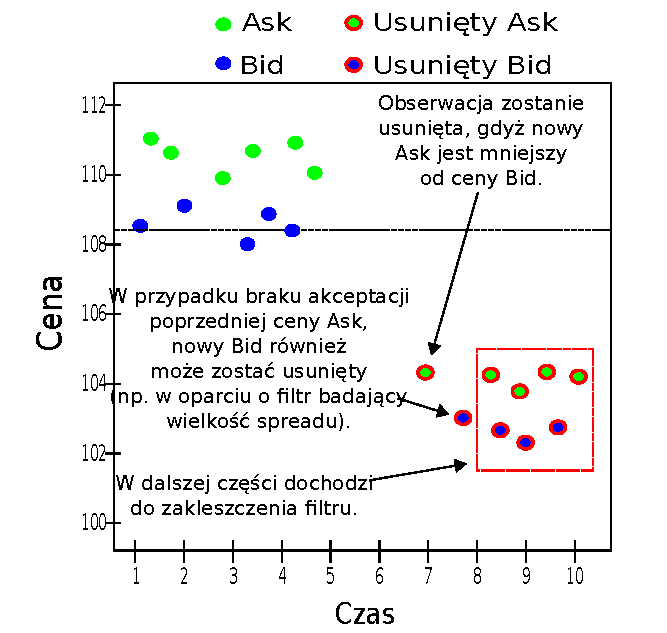
\includegraphics[width=0.6\textwidth]{wykresy/relacjaBIDASK.pdf}
%  \caption{Przypadek zakleszczenia się filtru spowodowany nagłym skokiem ceny.}
%  \label{fig:JUMP}
%\end{figure}

\subsection{Aktualizacja \MSpn}

Listing \ref{FiltrUpdate} przedstawia sposób aktualizacji średniego spreadu \MSpn:

\begin{algorithm}

\eIf{TickAccepted}
{ $\Delta t = t - lastTime$\\
\nlset{Uwaga 1}\label{uwg1ta}	$\phi = exp(\Delta t / \lambda)$\\
\nlset{Uwaga 2}\label{uwg2ta}	$\phi = max(\phi, \phi_{min})$\\
\nlset{Uwaga 3}\label{uwg3ta} 	$\phi = min(\phi, \phi_{max})$ \\ 
\nlset{Aktualizacja}\label{line:akt}	$\MSpn = \phi \cdot \MSpc + (1 - \phi) \Spt$
}
{
\nlset{Zabezpieczenie 3}\label{Zab3} \MSpn = \MSpc + RmVal\\
}


\caption{Algorytm aktualizacji \MSpn \label{FiltrUpdate}}
\end{algorithm}

Nowa wartość \MSpn jest ważoną średnią poprzedniej wartości i aktualnego spreadu. Przy czym  waga \Spt zależna jest od czasu pomiędzy dwiema ostatnimi obserwacjami (\ref{uwg1ta}). Im krótszy czas, tym wpływ nowej wartości spreadu jest większy. Dostosowywanie wartości $\phi$ odbywa się poprzez parametr $\lambda$ - większe wartości $\lambda$ oznaczają większy wpływ \Spt na wartość \MSpn. 

Dodatkowo wprowadzono parametr $\phi_{max}$, określający maksymalny udział aktualnego spreadu (\Spt) w \MSpn. Ma on na celu zapobieganie sytuacją zbytniego zmniejszenia się średniego spreadu gdy po dłuższym okresie jako pierwsze pojawi się tick którego spread względem starej przeciwnej ceny będzie bardzo mały, a spread dla następnych tików się powiększy, przez co kolejne obserwacje będą odrzucane, aż do momentu, odpowiedniego rozszerzenia się spreadu związnym z zabezpieczeniem \ref{Zab3}. W takiej sytuacji udział \Spt zostanie ograniczony do wartości $\phi_{max}$ Przykładowa sytuacja pokazana jest na rys. \ref{fig:deltaTime}. Jednocześnie należy zauważyć, że w pewnych przypadkach może to prowadzić do sytuacji w której spread będzie znacząco zawyżony. 

W tym przypadku ujawia się również dodatkowa słabość filtru mająca szczególne znaczenie w przypadku małej płynności instrumentu (rzadko pojawiających się danych). Dla pierwszej obserwacji po długim okresie spread może być liczony względem ceny która jest już nieaktualna, jednak nowa cena jeszcze się nie pojawiła \ref{fig:calcSpread}. W obecnym podejściu do fitracji danych, w którym założone jest działanie online (po sprawdzeniu tiku nie ma już do niego powrotu), obejście tego problemu jest bardzo trudne (o ile w ogóle możliwe). W pewnym stopniu rozwiązaniem jest wprowadzone wcześniej zabezpieczenie \ref{Zab1}, które nie dopuści do zakleszczenia się filtra, kosztem odrzucenia pierwszej obserwacji pojawiającej się po dłuższym okresie czasu (np. na otwarcie sesji).

Parametr $\phi_{min}$ określa minimalny udział \Spt w \MSpn. Przyspiesza on dostosowywanie się wartości średniego spreadu dla płynnego rynku. 

Linijka \ref{Zab3} jest kolejnym zabezpieczeniem przeciwko zakleszczeniu się filtru. Rozszerzenie spreadu o wartość $RmVal$ pozwala na samo-naprawienie się filtru w sytuacji w której nastąpił gwałtowny skok spreadu, kosztem kilku pierwszych obserwacji (por. \ref{fig:SpreadJump}). Takie zabezpieczenie posiada oczywistą wadę w przypadku całej serii złych danych - powolne rozszerzanie się średniego spreadu w końcu spowoduje, że obserwacje odstające zostaną uznane za poprawne (por \ref{fig:outSeries}). W tym przypadku należy dokonać wyboru dotyczącego wrażliwości filtru na długie serie złych danych, a szybkością samonaprawy w przypadku zakleszczenia. 

\bibliographystyle{plainnat}
\bibliography{literatura_mag}
\addcontentsline{toc}{section}{Bibliografia}
\listoftables
\addcontentsline{toc}{section}{Spis tabel}
\listoffigures
\addcontentsline{toc}{section}{Spis rysunków}
\printindex
\end{document}
